\documentclass[12pt, oneside, a4paper]{article}
\usepackage{ifpdf}
\usepackage{graphicx}
\usepackage[colorlinks,bookmarksopen,linkcolor=black,pdfauthor={Sharad,Prabhakar,Vikram},urlcolor=blue]{hyperref}
\usepackage[colorlinks,bookmarksopen]{hyperref}
\begin{document}
\begin{center}
\textbf{VISVESWARAYA TECHNOLOGICAL UNIVERSITY}
\end{center}
\begin{center}
\textbf{BELGAUM}\\
\thispagestyle{empty}
\begin{figure}[htb]
\begin{center}
\ifpdf
	
\includegraphics[scale=0.50]{vtu.png}
\else
%	
\includegraphics[scale=0.50]{vtu.png}
\fi
\end{center}
\end{figure}
\textbf{SRI JAYACHAMARAJENDRA COLLEGE OF ENGINEERING}
\textbf{MYSORE-570006}\\
\textsc{department of computer science and engineering}
\end{center}
\begin{figure}[htb]
\begin{center}
\ifpdf

\includegraphics[scale=0.30]{./logo.png}
\else
%	
\includegraphics[scale=0.30]{/home/prabhakar/logo.odg}
\fi
\end{center}
\end{figure}
\begin{center}
\textbf{\underline{Project on}}\\
\textsc{Generation of three address code for 'C' subset(Part 2).\\}
\emph{\\Guidance of}\\
\textbf{P.M.SHIVAMURTHY}\\
\textit{Lecturer}\\
\textit{Dept of CS$\&$E,SJCE Mysore.}\\
\end{center}
Team:
\begin{center}
\begin{tabular}{|c|c|c|}
\hline
%% row 1
\textsc{name}
&\textsc{roll no}
&\textsc{usn}
\\\hline
%% row 2
\textsc{vikram tv}
&61
&\textsc{4jc07cs120}
\\\hline
%% row 3
\textsc{prabhakar Gouda}
&37
&\textsc{4jc07cs070}
\\\hline
%% row 4
\textsc{sharad d}
&03
&\textsc{4jc06cs089}
\\\hline
\end{tabular}
\end{center}
\newpage
\thispagestyle{empty}
\tableofcontents
\newpage
\pagenumbering{arabic}

\section{Overview}

$\beta$ - parse language is the beta version of parsing of our own language.  It involves the best possibilities that we have seen from the classic language `C'.  Our language is purely a subset of the higher level language - 'C'.  The analysis phase of a compiler breaks up a source program into constituent pieces and produces an internal representation for it, called a intermediate code. Syntax-directed translation refers to a method of compiler implementation where the source language translation is completely driven by the parser. In other words, the parsing process and parse trees are used to direct semantic analysis and the translation of the source program. This can be a separate phase of a compiler or we can augment our conventional grammar with information to control the semantic analysis and translation. Such grammars are called attribute grammars.\\

\section{Glossary}
\begin{tabular}{ll}
%% row 1
$\beta$parse & Our own defined language.\\
source program & User program written in $\beta$parse spec.\\
keywords & The keywords supported by our language.\\
Symbol Table & The data structures that are used by parser and lexer to hold information.\\
Lexer & Scanner which finds the token and return to the parser.\\
Parser & Which handles the token.\\
SDT & Syntax directed translation.\\
IR & Intermediate representation.\\

\end{tabular}

\section{Flow diagram of the operation}
\begin{figure}[htb]
\begin{center}
\ifpdf
	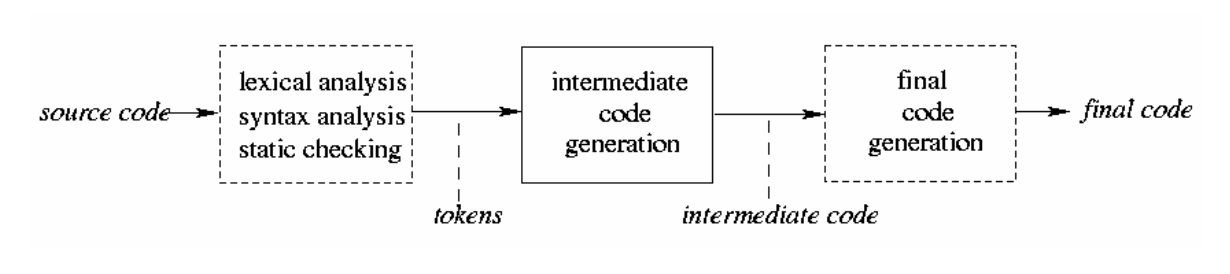
\includegraphics[scale=0.50]{snapshot6.png}
\else
%	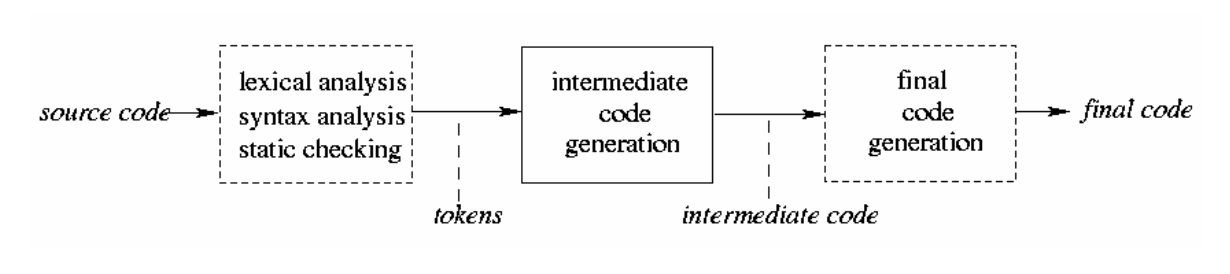
\includegraphics[scale=0.50]{snapshot6.png}
\fi
\caption{Operation}
\end{center}
\end{figure}

\section{Syntax-Directed Definitions and Translation Schemes}

When we associate semantic rules with productions, we use two notations:

\subsection{Syntax-Directed Definitions}
It give high-level specifications for translations. SDD hide many implementation details such as order of evaluation of semantic actions. We associate a production rule with a set of semantic actions, and we do not say when they will be evaluated.\\
When translating according to an SDT, it is normal not to construct the parse tree. Rather we perform actions as we parse; that is, we "go through the motions" of building the parse tree. To perform a translation that cannot be expressed by an SDT directly, it helps to build the parse tree first. For example, while we can translate infix to postfix by an SDT, we cannot translate to prefix. Define one or more attributes of each terminal and non terminal, and give rules relating the values of these translations at the various nodes of the parse tree.\\
\begin{itemize}
\item Rules can be associated with productions, because they relate translations at a node to translations at its parent and or children.\\
\item The rules for computing these translations together form a syntax-directed definition (SDD). Rules with no side effects (such as printing output) are called an attribute grammar.
\end{itemize}

\section{Intermediate Representation}
Most compilers translate the source program first to some form of intermediate representation and convert from there into machine code. The intermediate representation is a machine- and language-independent version of the original source code. Although converting the code twice introduces another step, use of an intermediate representation provides advantages in increased abstraction, cleaner separation between the front and back ends, and adds possibilities for re-targeting/cross-compilation. Intermediate representations also lend themselves to supporting advanced compiler optimizations and most optimization is done on this form of the code.

\begin{itemize}
\item An abstract machine language and independent of source language
\item Expresses operations of target machine and not specific to any particular machine
\end{itemize}

\section{Example}
Consider the typical example,
\begin{figure}[htb]
\begin{center}
\ifpdf
	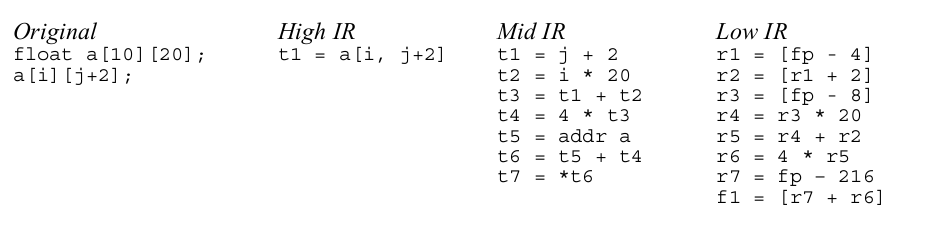
\includegraphics[scale=0.450]{./snapshot7.png}
\else
%	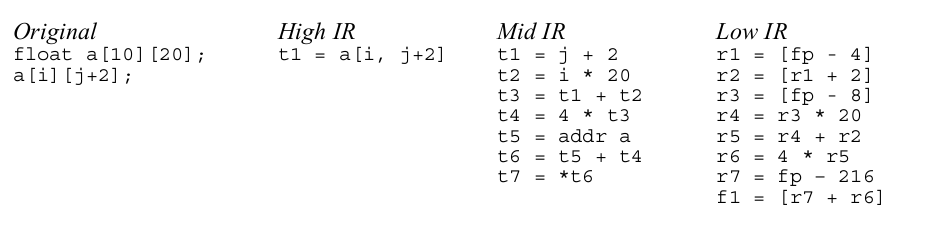
\includegraphics[scale=0.50]{./snapshot7.png}
\fi
\caption{Example}
\end{center}
\end{figure}


\section{Three Address Code}
Three-address code (TAC) will be the intermediate representation used in our Decaf compiler. It is essentially a generic assembly language that falls in the lower-end of the mid-level IRs. Some variant of 2, 3 or 4 address code is fairly commonly used as an IR, since it maps well to most assembly languages.

A TAC instruction can have at most three operands. The operands could be two operands to a binary arithmetic operator and the third the result location, or an operand to compare to zero and a second location to branch to, and so on. For example, below on the left is an arithmetic expression and on the right, is a translation into TAC instructions:

\begin{figure}[htb]
\begin{center}
\ifpdf
	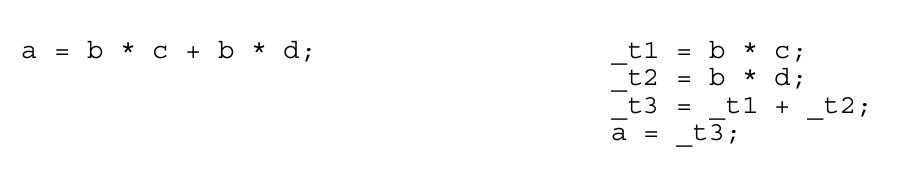
\includegraphics[scale=0.50]{./snapshot8.png}
\else
%	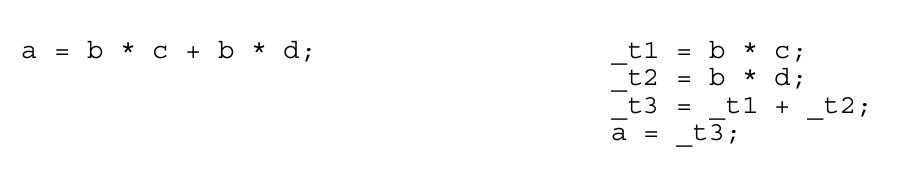
\includegraphics[scale=0.50]{./snapshot8.png}
\fi
\caption{Example three address code}
\end{center}
\end{figure}

\section{Implementation of Translation Schemes}
It indicate the order of evaluation of semantic actions associated with a production rule. In other words, translation schemes give a little bit information about implementation details.

\subsection{Translation of Expressions}
\begin{tabular}{ll}
PRODUCTION &SEMANTIC RULES\\\\
\emph{S $\rightarrow$ \textbf{id} $=$ E;} & \emph{S.code $=$ E.code}\\
& \emph{gen(top.get(\textbf{id}.lexeme) '=' E.addr)}\\\\

\emph{E $\rightarrow$ E1 + E2}	& \emph{E.addr = \textbf{new} Temp()}\\
& \emph{E.code = E1.code $\|$ E2.code $\|$}\\
& \emph{gen(E.addr'='E1.addr '+' E2.addr}\\\\
\emph{E $\rightarrow$ E1 - E2}	& \emph{E.addr = \textbf{new} Temp()}\\
& \emph{E.code = E1.code $\|$ E2.code $\|$}\\
& \emph{gen(E.addr'='E1.addr '-' E2.addr}\\\\
\emph{E $\rightarrow$ E1 * E2}	& \emph{E.addr = \textbf{new} Temp()}\\
& \emph{E.code = E1.code $\|$ E2.code $\|$}\\
& \emph{gen(E.addr'='E1.addr '*' E2.addr}\\\\
\emph{E $\rightarrow$ E1 / E2}	& \emph{E.addr = \textbf{new} Temp()}\\
& \emph{E.code = E1.code $\|$ E2.code $\|$}\\
& \emph{gen(E.addr'='E1.addr '/' E2.addr}\\\\
$|$ \emph{-E}& \emph{E.addr = \textbf{new} Temp()}\\
&\emph{E.code = E2.code $\|$}\\
&\emph{E.addr $'='$\textbf{minus}E1.addr}\\\\
$|$ \emph{(E1)}& \emph{E.addr = E1.addr}\\
& \emph{E.code = E1.code}\\\\
$|$ \textbf{id}& \emph{E.addr = top.get(\textbf{id}),lexeme)}\\
& \emph{E.code = ''}\\\\
\end{tabular}

Syntax directed definition in the above case builds up the three-address code for an assignment statement S using attribute \emph{code} for S and \emph{addr} and \emph{code} for an expression E. Attribute \emph{S.code} and \emph{E.code} denotes the three address code for S and E respectively. Attribute \emph{E.addr} denotes the address that will hold the value of E.  Here, '*' and '/' have higher precedence than '+' and '-'.\\

Consider the last production \emph{E$\rightarrow$ \textbf{id}} in the above definition , the semantic rules for the this production define E.addr to point to the symble table entry for this instance if \textbf{id}. Let top denotes the current symble table. Function \emph{top.get} retrieves the entry when it is applied to the string represents \textbf{id.}lexeme of this instance of \textbf{id}.\\

\subsection{Flow of control statements}
We assume that \emph{newlabel()} creates a new label each time it is called, and that \emph{L} attaches label L to the next three address instruction to be generated.\\

A program consists of a statement generated by \emph{P$\rightarrow$ S}. The semantic rules associated with this production initializes \emph{S.next} to a new label. The token \textbf{assign} in the production \emph{S$\rightarrow$\textbf{assign}} is a place holder for assignment statements.

In translating \emph{S$\rightarrow$ \textbf{if}( B ) S1}, the semantic rule create a new label \emph{B.true} and attach it to the first three address instruction generated for the statement S1. Thus , jumps to B.true with in code code for B will go to code S1.\\

In the translating \emph{S$\rightarrow$ \textbf{if} ( B ) S1 \textbf{else} S2}, the code for the boolean expression B jumps out of it to the first instruction of the code for S1 if B is true, and to the first instruction of the code for S2 if b is false.

\begin{tabular}{ll}
\textbf{PRODUCTIONS}& \textbf{SEMANTIC RULES}\\\\
\emph{P $\rightarrow$S }& \emph{S.next = newlabel()}\\
& \emph{P.code = S.code$\|$ label(S.next)}\\\\
\emph{S $\rightarrow$ \textbf{assign}}& \emph{S.code = \textbf{assign}.code}\\\\
\emph{S $\rightarrow$ \textbf{if}( B )S1}& \emph{B.true = newlabel()}\\
& \emph{B.false = S1.next = S.next}\\
& \emph{S.code = B.code $\|$ label(B.true)$\|$ S1.code}\\\\
\emph{S $\rightarrow$ \textbf{if}( B ) S1 \textbf{else} S2}& \emph{B.true = newlabel()}\\
&\emph{B.false = newlabel()}\\
&\emph{S1.next = S2.next = S.next}\\
&\emph{S.code = B.code}\\
& \emph{$\|$label(B.true)$\|$S1.code  }\\
&\emph{gen ( '\textbf{goto}' S.next)}\\
& \emph{label(B.false) $\|$ S2.code}\\\\
\emph{S $\rightarrow$ \textbf{while}( B ) S1}& \emph{begin = newlabel()}\\
& \emph{B.true = newlabel()}\\
&\emph{B.false = s.next}\\
&\emph{S1.next = begin}\\
&\emph{S.code = label(begin) $\|$ B.code}\\
&\emph{$\|$ label(B.true) $\|$ S1.code}\\
&\emph{gen ('\textbf{goto}' begin)}\\\\
\emph{S $\rightarrow$ S1S2}& \emph{S1.next = newlabel()}\\
&\emph{S2.next = S.next}\\
&\emph{S.code = S1.code $\|$ label(S1.next)$\|$ S2.code}\\\\
\end{tabular}

\subsection{Control-Flow Translation of Boolean Expression}
The semantic rules for Boolean expression shown below.\\
The Boolean expression B is translated into three address instruction that evaluate B using Condition and unconditional jumps to one of two labels: B.true if true and B.false if false.\\


\begin{tabular}{ll}
\textbf{PRODUCTION}& \textbf{SEMANTIC RULES}\\\\
\emph{B $\rightarrow$ B1 $\|$ B2}& \emph{B1.true = B.true}\\
&\emph{B1.false = newlabel()}\\
&\emph{B2.true = B.true}\\
& \emph{B2.false = B.false}\\
&\emph{B.code = B1.code $\|$ label( B1.false ) $\|$ B2.code }\\\\
\emph{B $\rightarrow$ B1 $\&\&$ B2}& \emph{B1.true = newlabel()}\\
&\emph{B1.false = B.false}\\
&\emph{B2.true = B.true }\\
&\emph{B2.false = B.false}\\
&\emph{B.code = B1.code $\|$ label( B1.true ) $\|$ B2.code}\\\\
\emph{B $\rightarrow$ !B1}& \emph{B1.true = B.false}\\
&\emph{B1.false = B.true}\\
&\emph{B.code = B1.code}\\\\
\emph{B $\rightarrow$ E1 \textbf{rel} E2}&\emph{B.code = E1.code $\|$ E2.code}\\
& $\|$\emph{gen('\textbf{if}' E1.addr \textbf{rel}.op E2.addr '\textbf{goto}' B.true)}\\
& $\|$ \emph{gen(\textbf{'goto'} B.false)}\\\\
\emph{B $\rightarrow$ \textbf{true}}& \emph{B.code = gen(\textbf{'goto'} B.true)}\\\\
\emph{B $\rightarrow$\textbf{false}}& \emph{B.code = gen (\textbf{'goto'} B.false)}\\\\

\end{tabular}

The remaining productions for B are translated as follows.
\begin{itemize}
\item Suppose B is the form B1$\|$B2. If B1 is true, then we immediately know that B itself is true, so B1.true.\\
\item The translation of B1 $\&$ B2 is similar.\\
\item No code is needed for expression B of the form !B1 just interchange the true and false exists of B to get the true and false exists of B1.\\
\item the constants \textbf{true} and \textbf{false} translate into jumps to B.true and B.false, respectively.\\
\end{itemize}
 
The semantics for the expressions,  control flow statements and boolean values in their context are suitably implemented.

\section{References}
\begin{itemize}
\item Lex and Yacc by John R. Levine, Tony Mason, Doug Brown - O’Reilly Publications
\item A Compact Guide to Lex and Yacc by Tom Niemann at \href{http://epaperpress.com}{epaperpress.com}
\item Compilers Principles Techniques and Tools by Afred V.Aho, Monica S.lam, Ravi Sethi,Jeffrey D.Ullman
\item \href{http://en.wikipaedia.org/wiki/Syntax analysis}{Wikipaedia}
\end{itemize}


\end{document}